\documentclass[10pt,a4paper]{article}

\usepackage[utf8]{inputenc}
\usepackage[T1]{fontenc}
\usepackage[spanish]{babel}
\usepackage[top=2cm,bottom=2cm,left=2cm,right=2cm]{geometry}
\usepackage{graphicx}
\usepackage{booktabs}
\usepackage{multirow}
\usepackage{subcaption}
\usepackage{caption}
\usepackage{placeins}
\usepackage{microtype}
\usepackage{amsmath}
\usepackage[numbers,sort&compress]{natbib}
\usepackage[hidelinks]{hyperref}

\captionsetup{font=small,labelfont=bf,skip=4pt}
\setlength{\parskip}{2pt}
\setlength{\parindent}{0pt}
\renewcommand{\arraystretch}{1.08}
\renewcommand{\topfraction}{0.85}
\renewcommand{\bottomfraction}{0.85}
\renewcommand{\textfraction}{0.1}
\renewcommand{\floatpagefraction}{0.7}

% Nombres de variables en tipo máquina (admite guiones bajos)
\newcommand{\var}[1]{\texttt{\detokenize{#1}}}

\title{Explicabilidad de un modelo de scoring de crédito:\\ qué pesa, si nos fiamos y qué hacer con ello}
\author{Guzmán Ignacio Pérez Ibarz \\ Explainable AI, proyecto final, ICAI Comillas, 2026/27}
\date{\today}

\begin{document}
\maketitle

\begin{abstract}
\noindent He entrenado un XGBoost que predice si un cliente de tarjeta de crédito va a dejar de pagar el mes siguiente y lo he explicado con SHAP, importancia por permutación, PDP/ICE y LIME. Después compruebo si esas explicaciones son fiables (cinco sanity checks) y las uso para tres cosas: simplificar y mejorar el modelo, sacar conclusiones de negocio y auditar la equidad. El modelo llega a 0,773 de AUC en test frente a 0,714 de una regresión logística. El historial reciente de pagos domina todas las explicaciones, SHAP pasa los chequeos y LIME es el punto débil. Código: .
\end{abstract}

%------------------------------------------------------------------
\section{Introducción}
El problema es de clasificación binaria: con los datos de un cliente y su historial de seis meses hay que predecir si no va a pagar el mes siguiente (\var{default}=1). Es riesgo de crédito de manual y aquí no basta con que el modelo acierte, porque hay tres partes a las que les importa entender por qué. El analista de riesgos necesita saber por qué se marca a un cliente para fiarse del modelo o corregirlo. El cliente tiene derecho a una explicación y a saber qué podría cambiar. Y el regulador pide transparencia: evaluar la solvencia de personas físicas es sistema de alto riesgo en la Ley de IA europea \citep{aiact}, el RGPD limita las decisiones totalmente automatizadas \citep{gdpr} y el TJUE ha dicho que generar una puntuación de crédito puede ser una de ellas \citep{schufa}. Las fechas de aplicación de la Ley de IA han ido cambiando así que no las pongo.

Mis objetivos son tres: ver qué criterios pesan más en la predicción, comprobar si me puedo fiar de esas explicaciones y usarlas para mejorar el modelo, sacar conclusiones de negocio y revisar si trata distinto a distintos grupos.

%------------------------------------------------------------------
\section{Datos y métodos}
\subsection{Datos}
Uso el dataset Default of Credit Card Clients de UCI \citep{uci350}, de un banco de Taiwán entre abril y septiembre de 2005 \citep{yeh2009}. Tiene 30\,000 clientes y 23 variables: límite de crédito (\var{LIMIT_BAL}), sexo, educación, estado civil, edad, estado de pago de cada uno de los seis meses (\var{PAY_0}, \var{PAY_2} a \var{PAY_6}), importe de la factura (\var{BILL_AMT1} a \var{BILL_AMT6}) e importe pagado (\var{PAY_AMT1} a \var{PAY_AMT6}). Lo que se predice es el impago del mes siguiente.

El preprocesado es mínimo. Quito 35 filas duplicadas (quedan 29\,965), agrupo en ``otros'' los códigos de \var{EDUCATION} y \var{MARRIAGE} que no salen en la descripción oficial (5, 6 y 0 por ejemplo) y no hay nulos. La tasa de impago es del 22,1\,\%, o sea hay desbalanceo y no tiene sentido mirar solo la accuracy. Otra pega es que UCI solo define \var{PAY}=$-1$ (pago a tiempo) y de 1 a 9 (meses de retraso) pero en los datos aparecen también $-2$ y 0 sin explicar, y lo dejo como limitación. El sexo es un atributo sensible así que no entra como variable del modelo, lo guardo aparte para auditar (sección~\ref{sec:equidad}). La partición es estratificada 60/20/20 (17\,979 / 5\,993 / 5\,993) con la misma tasa de impago en las tres. Como solo hay un corte temporal una partición aleatoria me parece razonable.

\begin{figure}[htbp]
  \centering
  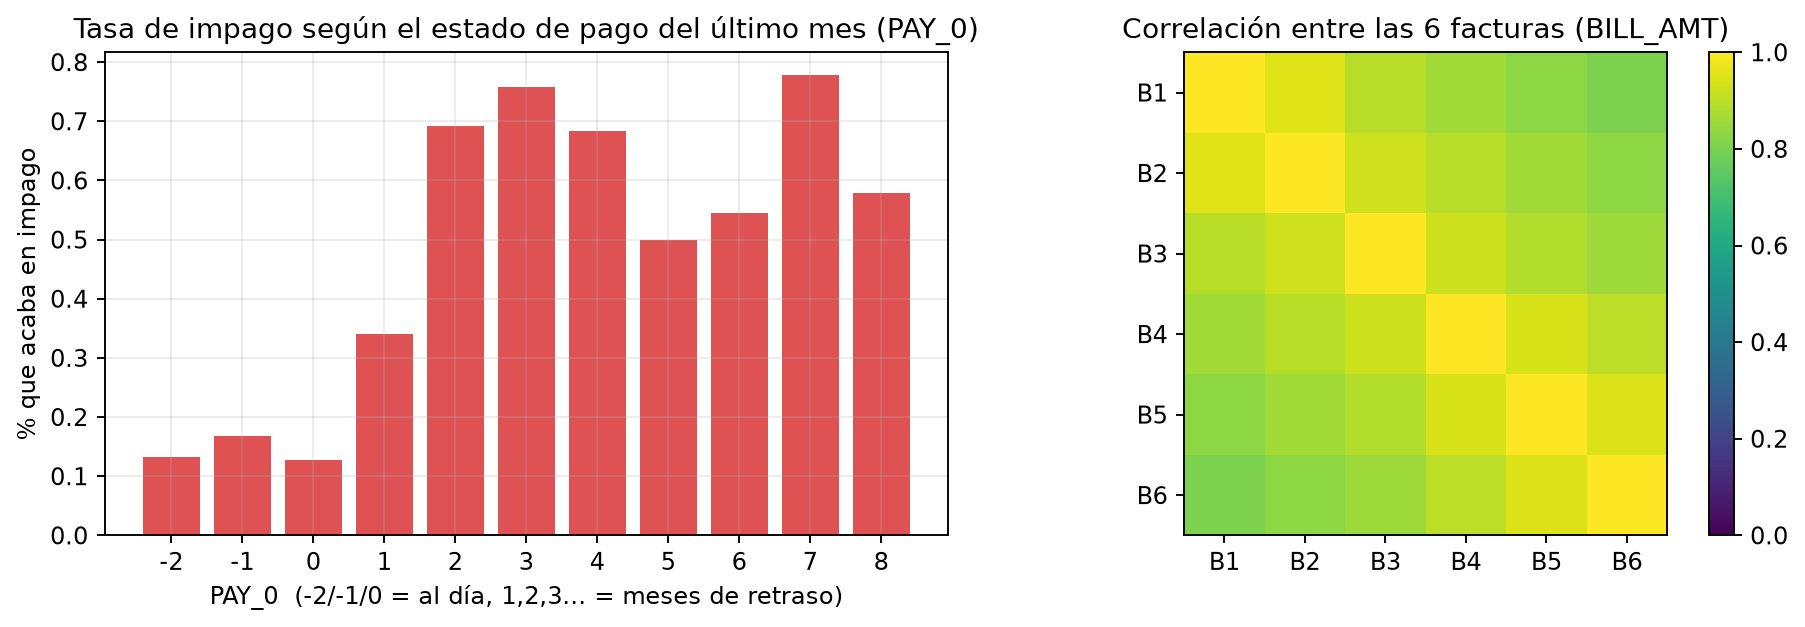
\includegraphics[width=0.9\linewidth]{figures/01_eda.png}
  \caption{Izquierda: tasa de impago según el estado de pago del último mes (\var{PAY_0}). Derecha: correlación entre las seis facturas (media 0,89).}
  \label{fig:eda}
\end{figure}

\subsection{Modelos y evaluación}
Comparo un baseline tonto (dummy, que predice la tasa base), una regresión logística estandarizada y XGBoost \citep{chen2016}. En XGBoost pruebo cinco configuraciones de poca profundidad con early stopping sobre validación y me quedo con la de mejor AUC de validación (profundidad 4, tasa de aprendizaje 0,05, 139 árboles). Entre configuraciones hay unas 0,002 de diferencia de AUC así que la elección no es muy fuerte. Las métricas son ROC-AUC, PR-AUC, Brier y F1, precisión y recall con el umbral que maximiza el F1 en validación. Para el sobreajuste miro la diferencia entre train, validación y test, una validación cruzada de 5 folds y un intervalo bootstrap del AUC de test. El test solo lo uso para los números finales.

\subsection{Técnicas de explicabilidad}
\begin{itemize}\setlength\itemsep{1pt}
  \item SHAP (TreeSHAP) \citep{lundberg2017,lundberg2020}: global y local, es exacto y rápido en árboles y va en log-odds. Es la técnica principal.
  \item Importancia por permutación y ganancia de XGBoost: dos medidas globales para contrastar SHAP. PDP/ICE para ver la forma del efecto de cada variable.
  \item LIME \citep{ribeiro2016}: explicación local independiente de SHAP para ver si coinciden. Además hago un contrafactual casero de qué pasaría si cambio a mano variables de un cliente \citep{wachter2018}.
  \item Cinco sanity checks \citep{adebayo2018}: aditividad de SHAP, etiquetas barajadas, barajar las variables top frente a barajar al azar, acuerdo con LIME y estabilidad con reentrenos bootstrap.
\end{itemize}

%------------------------------------------------------------------
\section{Resultados}
\subsection{Rendimiento del modelo}
Según la tabla~\ref{tab:modelos} XGBoost le saca bastante a la regresión logística (0,773 frente a 0,714 de AUC y también mejora en PR-AUC y Brier), y yo esperaba que estuvieran más cerca. Mi hipótesis, que no he comprobado, es que la logística trata \var{PAY_*} como lineal cuando el efecto real es un escalón (sección~\ref{sec:global}). El sobreajuste es leve: el AUC baja de 0,816 en train a 0,787 en validación y 0,773 en test, la validación cruzada da $0{,}785\pm0{,}005$ y el IC95\,\% bootstrap del test es [0,758; 0,787]. La calibración es buena (figura~\ref{fig:modelo}). Con el umbral de 0,27 detecta el 56\,\% de los impagos pero la mitad de sus alertas son falsas alarmas, así que sirve pero no es espectacular.

\begin{table}[htbp]
\centering\small
\caption{Métricas en test (umbral que maximiza el F1 en validación).}\label{tab:modelos}
\begin{tabular}{lrrrrrrr}
\toprule
Modelo & ROC-AUC & PR-AUC & Brier & F1 & Precisión & Recall & Umbral \\
\midrule
Dummy & 0,500 & 0,221 & 0,172 & 0,362 & 0,221 & 1,000 & 0,05 \\
Regresión logística & 0,714 & 0,504 & 0,146 & 0,493 & 0,537 & 0,456 & 0,29 \\
XGBoost & 0,773 & 0,555 & 0,136 & 0,535 & 0,513 & 0,558 & 0,27 \\
\bottomrule
\end{tabular}
\end{table}

\begin{figure}[htbp]
  \centering
  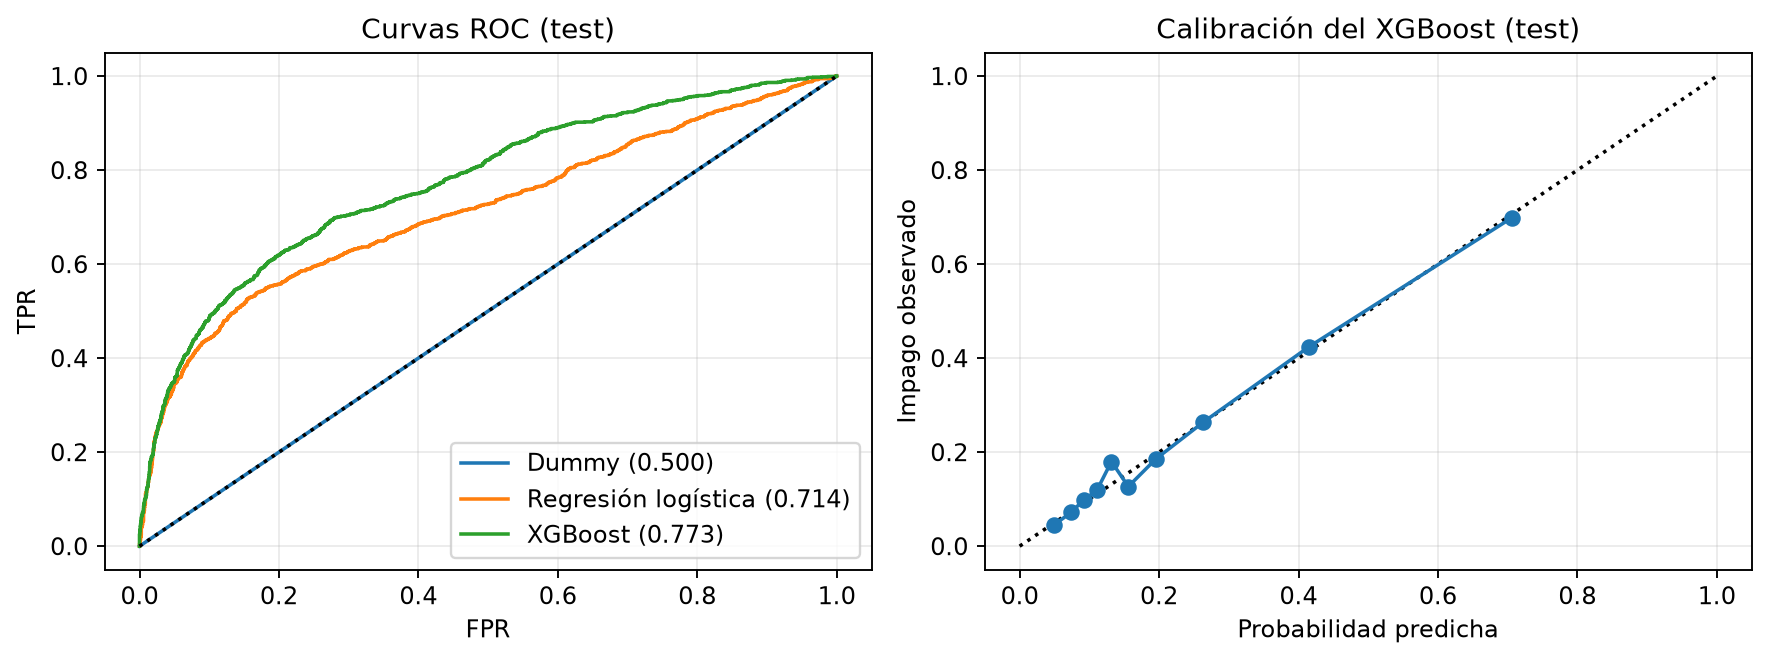
\includegraphics[width=0.85\linewidth]{figures/02_modelo.png}
  \caption{Curvas ROC en test (izquierda) y calibración del XGBoost (derecha).}
  \label{fig:modelo}
\end{figure}

\subsection{Explicaciones globales}\label{sec:global}
\var{PAY_0} manda con diferencia (mean$|$SHAP$|$ de 0,48 frente a 0,16 de la segunda). Detrás vienen \var{LIMIT_BAL}, \var{BILL_AMT1} y \var{PAY_2} y luego los importes pagados: pagar más y tener más límite baja el riesgo y los retrasos lo suben hasta más de $+2$ en log-odds (figura~\ref{fig:shap}). Los tres rankings (SHAP, permutación y ganancia) se parecen bastante (Spearman de 0,79, 0,88 y 0,74) y cuatro de las cinco primeras variables coinciden entre SHAP y permutación (tabla~\ref{tab:imp}). Lo que más chirría es \var{PAY_2}, segunda por ganancia pero con poca caída de AUC al permutarla. Mi hipótesis, sin comprobar, es que está muy relacionada con \var{PAY_0} y el modelo se apoya en una cuando se baraja la otra.

\begin{figure}[htbp]
  \centering
  \begin{subfigure}{0.52\linewidth}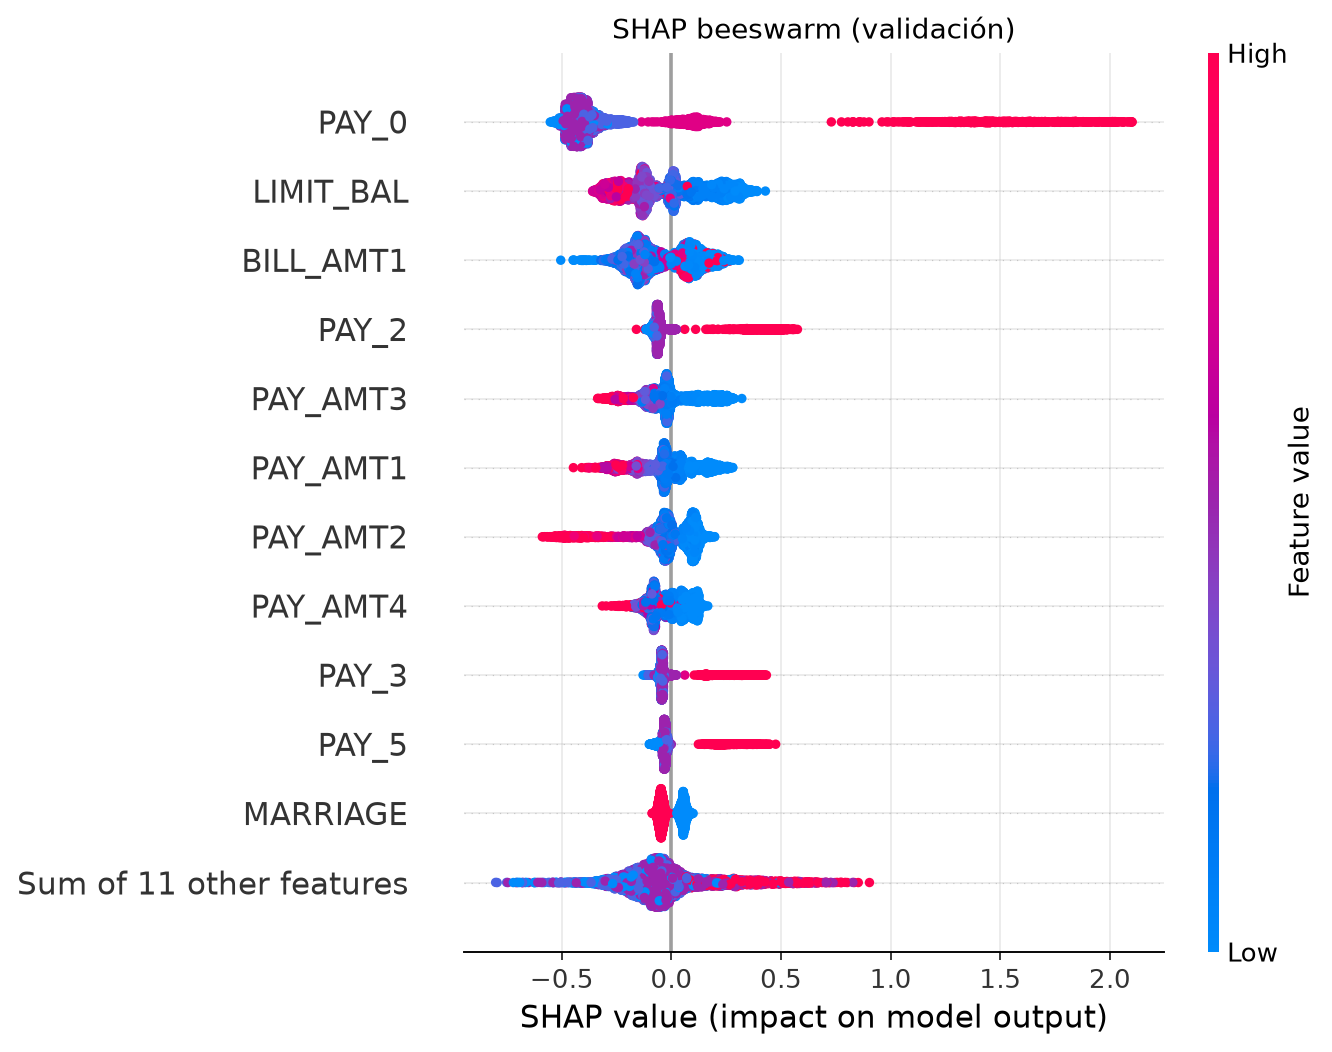
\includegraphics[width=\linewidth]{figures/03_shap_beeswarm.png}\end{subfigure}\hfill
  \begin{subfigure}{0.46\linewidth}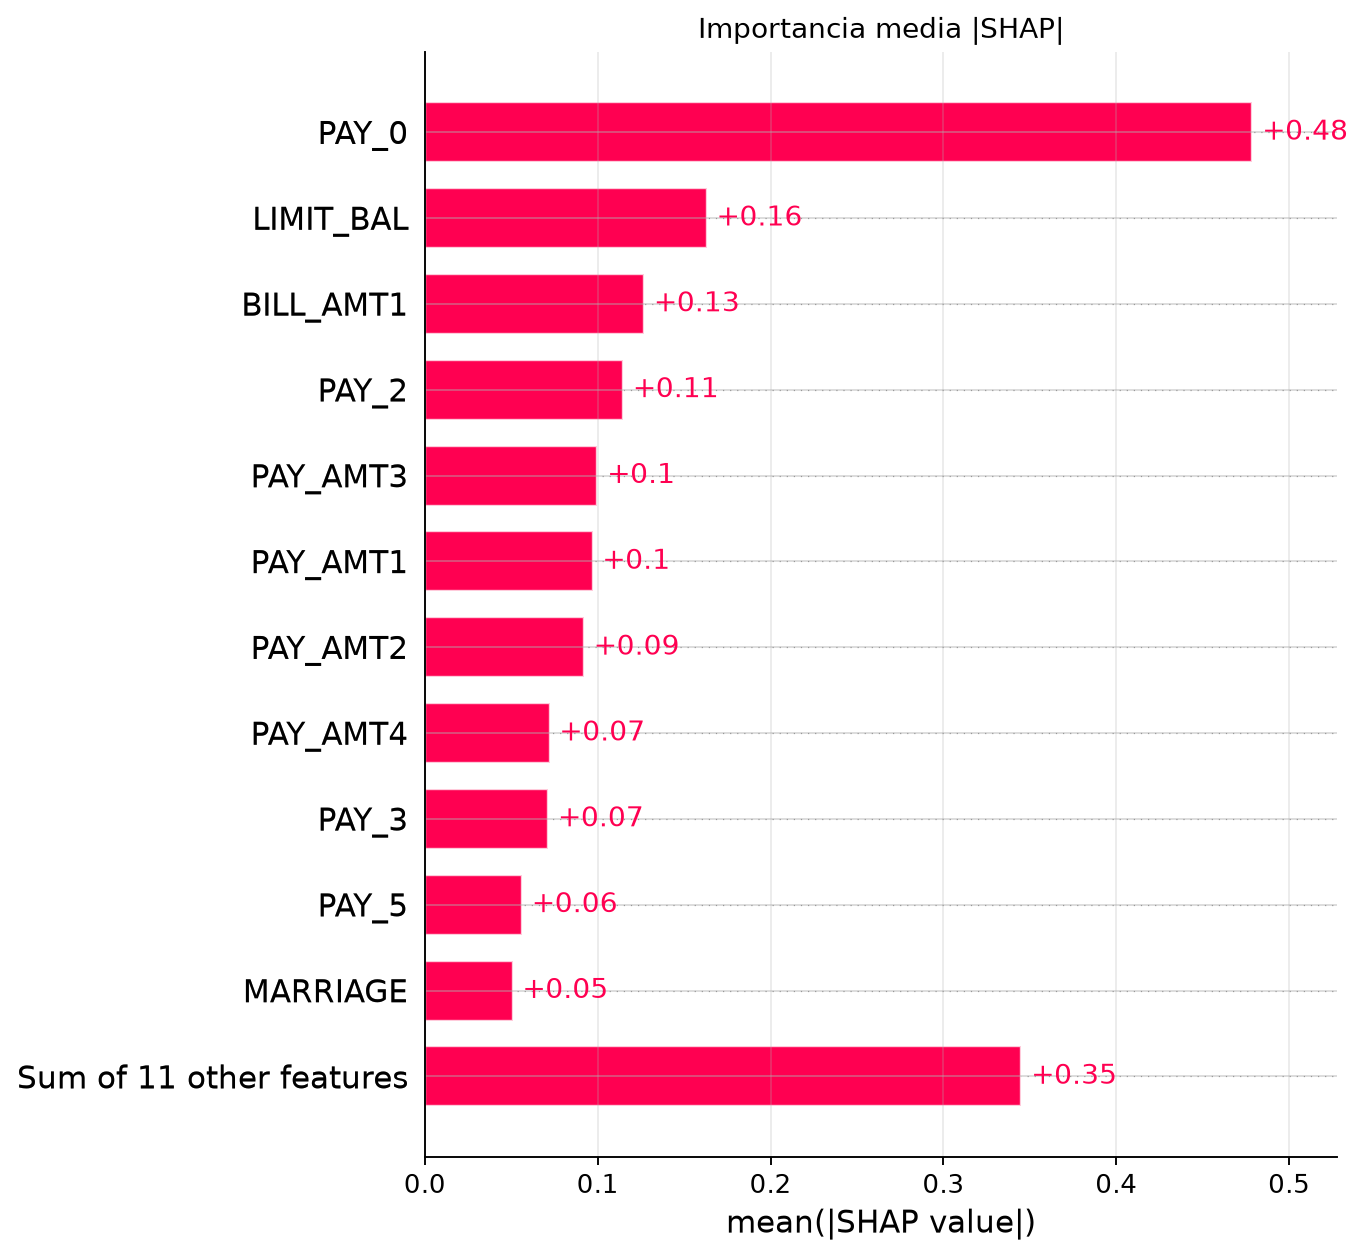
\includegraphics[width=\linewidth]{figures/03_shap_bar.png}\end{subfigure}
  \caption{SHAP global en validación: beeswarm (izquierda) e importancia media $|$SHAP$|$ (derecha).}
  \label{fig:shap}
\end{figure}

\begin{table}[htbp]
\centering\small
\caption{Importancia de las variables principales (validación).}\label{tab:imp}
\begin{tabular}{lrrr}
\toprule
Variable & mean$|$SHAP$|$ & Permutación (caída AUC) & Ganancia XGBoost \\
\midrule
\var{PAY_0} & 0,479 & 0,0746 & 17\,661 \\
\var{LIMIT_BAL} & 0,163 & 0,0156 & 1\,823 \\
\var{BILL_AMT1} & 0,127 & 0,0149 & 1\,791 \\
\var{PAY_2} & 0,115 & 0,0058 & 5\,650 \\
\var{PAY_AMT3} & 0,100 & 0,0039 & 1\,578 \\
\var{PAY_AMT1} & 0,097 & 0,0045 & 1\,617 \\
\var{PAY_AMT2} & 0,092 & 0,0035 & 1\,438 \\
\var{PAY_AMT4} & 0,072 & 0,0009 & 1\,130 \\
\bottomrule
\end{tabular}
\end{table}

El PDP de \var{PAY_0} (figura~\ref{fig:pdp}) es un escalón: el riesgo medio es 0,17 hasta 0, sube a 0,22 con un mes de retraso y salta a 0,57 con dos, y ya no cambia (para el modelo dos meses de retraso son lo mismo que ocho). Las ICE son casi paralelas. En \var{LIMIT_BAL} el riesgo baja de 0,26 a 0,20 hasta unos 150\,000 y luego se aplana, pero las ICE son muy distintas entre clientes así que el PDP medio esconde interacciones. El salto raro cerca de 360\,000 lo atribuyo a que hay pocos datos ahí. Tampoco hay que leer \var{LIMIT_BAL} como causal porque lo fija el propio banco según lo que opina del cliente.

\begin{figure}[htbp]
  \centering
  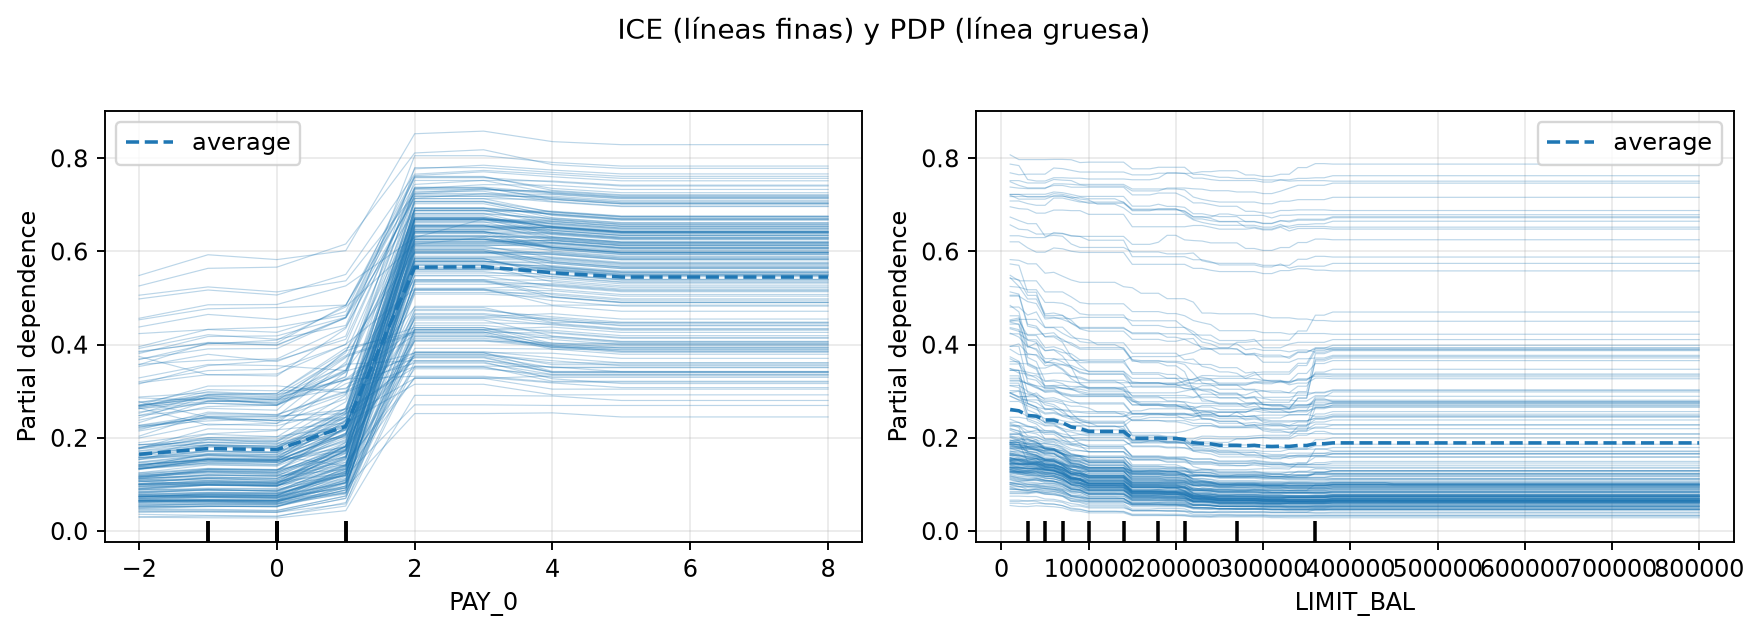
\includegraphics[width=0.85\linewidth]{figures/04_pdp_ice.png}
  \caption{PDP (línea gruesa) e ICE (líneas finas) de \var{PAY_0} y \var{LIMIT_BAL}.}
  \label{fig:pdp}
\end{figure}

\subsection{Explicaciones locales}
Miro tres clientes de validación (figura~\ref{fig:waterfall}). En el verdadero positivo (P=0,85) casi todo lo ponen \var{PAY_0}=2 ($+1{,}4$ en log-odds) y \var{PAY_2}=2 ($+0{,}35$). Me llama la atención que \var{BILL_AMT1} sea baja y aun así sume riesgo, lo que sugiere que su efecto depende del resto del cliente. En el falso negativo (P=0,03) todo empuja a la baja (\var{PAY_0}=$-2$, pagos grandes, límite de 200\,000) y el cliente impagó igual. La explicación dice por qué el modelo estaba tan seguro pero no por qué falló, y seguramente falta información que no está en los datos. El falso positivo (P=0,85) es casi idéntico al verdadero positivo, con dos meses de retraso en los seis meses, y no impagó. Son dos clientes con la misma explicación y distinto resultado, que es el límite de lo que se puede sacar con estas variables.

\begin{figure}[htbp]
  \centering
  \begin{subfigure}{0.33\linewidth}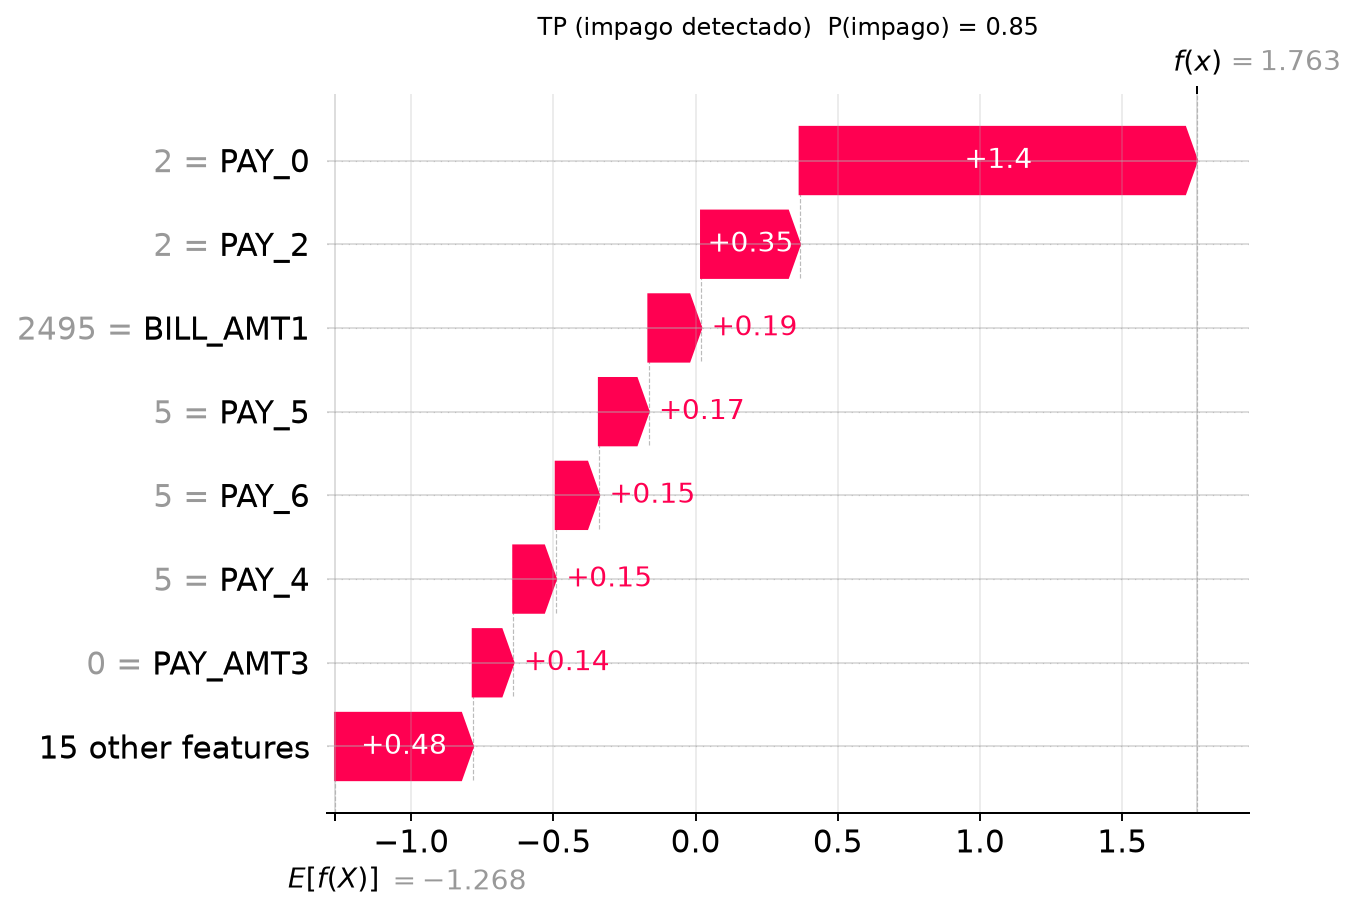
\includegraphics[width=\linewidth]{figures/05_waterfall_tp.png}\caption{Verdadero positivo}\end{subfigure}\hfill
  \begin{subfigure}{0.33\linewidth}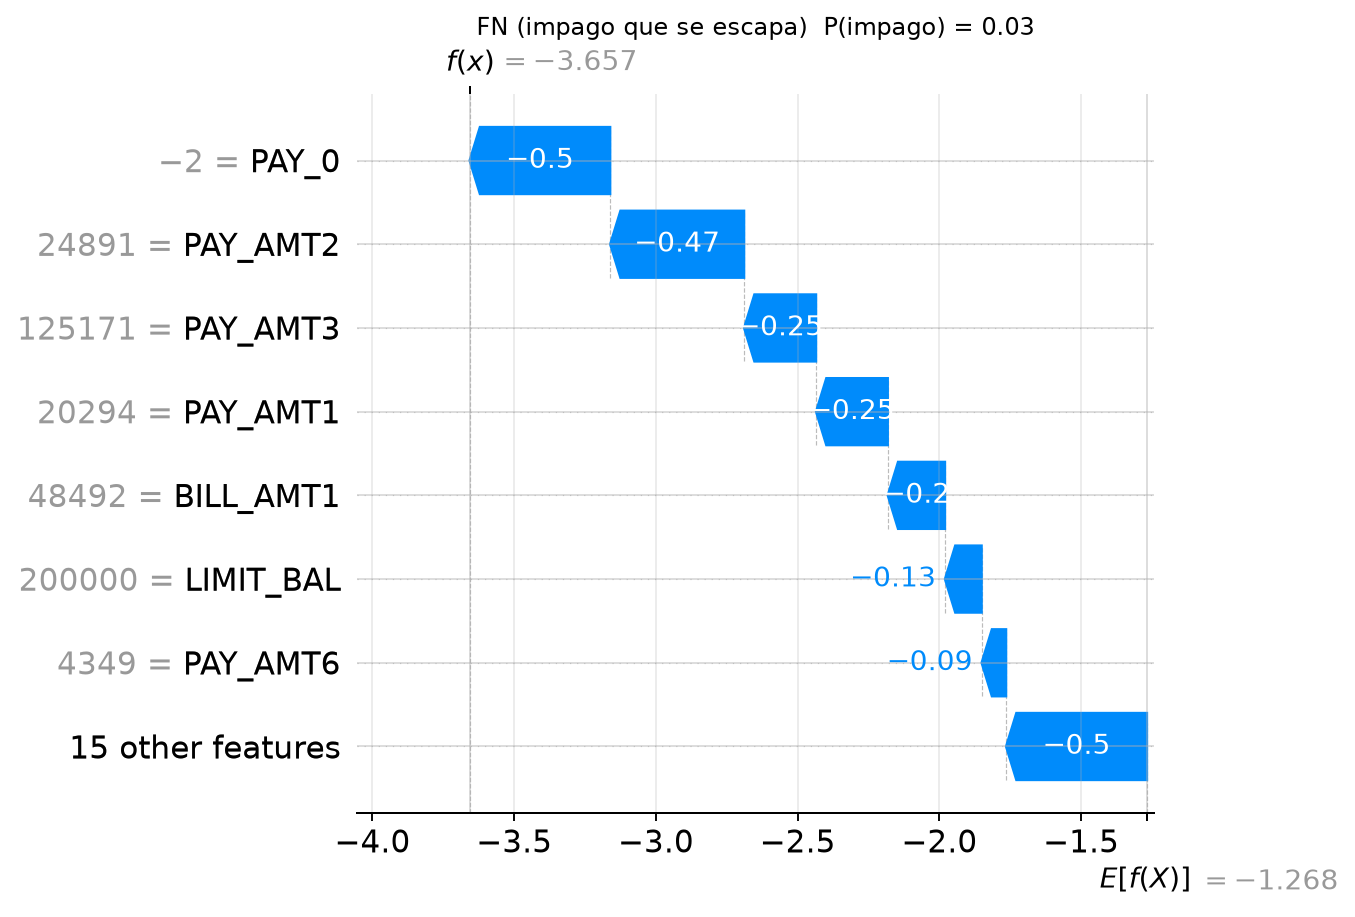
\includegraphics[width=\linewidth]{figures/05_waterfall_fn.png}\caption{Falso negativo}\end{subfigure}\hfill
  \begin{subfigure}{0.33\linewidth}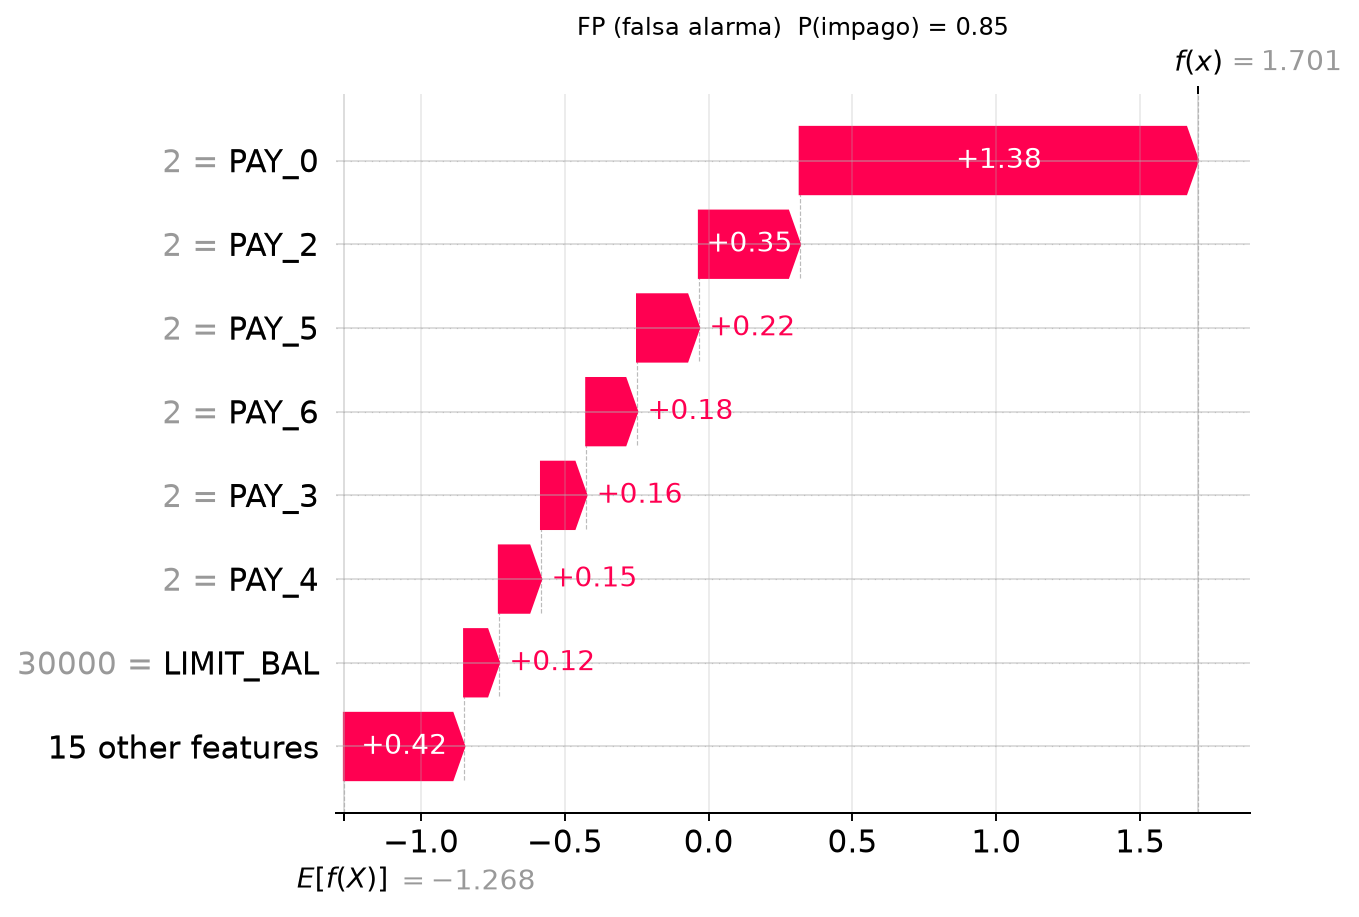
\includegraphics[width=\linewidth]{figures/05_waterfall_fp.png}\caption{Falso positivo}\end{subfigure}
  \caption{Explicaciones locales SHAP (log-odds). La base es $-1{,}27$ (22\,\% de impago).}
  \label{fig:waterfall}
\end{figure}

LIME y SHAP coinciden en que \var{PAY_0} es la primera variable en los tres casos pero en el resto del top-5 solo comparten 2, 3 y 4 de 5. LIME mete \var{LIMIT_BAL} y \var{BILL_AMT4} donde SHAP pone otras, y tiene sentido porque LIME ajusta un modelo lineal local sobre perturbaciones discretizadas mientras que SHAP reparte exactamente la predicción del árbol.

Para el contrafactual casero cojo primero un cliente justo por encima del umbral (P=0,27) y cualquier cambio pequeño lo saca de la lista: pagar el doble lo deja en 0,25, deber la mitad en 0,26, pagar cinco veces más en 0,15 y haber pagado a tiempo el último mes en 0,16. Con un cliente de riesgo alto (el verdadero positivo, P=0,85) ninguna acción lo saca. Tiene los seis pagos a 0 así que pagar $\times5$ no cambia nada ($0\times5=0$) y probé con un pago fijo de 20\,000 al mes (0,66), deber la mitad (0,79) y \var{PAY_0}=0 (0,59), todos por encima del umbral de 0,27. Las acciones solo le dan la vuelta al modelo cuando el cliente ya está cerca del umbral. Son pruebas manuales, una variable cada vez, así que las tomo como pista y no como conclusión.

\subsection{¿Son fiables las explicaciones?}
La tabla~\ref{tab:sanity} resume los cinco chequeos. SHAP los supera: cumple la aditividad, colapsa con etiquetas barajadas y barajar sus cinco variables top baja el AUC en 0,13 frente a 0,03 al azar (figura~\ref{fig:topk}). El punto débil es LIME, con un solape del top-3 de solo 0,64 en 30 clientes. La estabilidad es buena arriba del ranking (el top-5 se repite en un 90\,\% de los reentrenos) y peor en la cola (Spearman medio de 0,82).

\begin{table}[htbp]
\centering\small
\caption{Sanity checks de las explicaciones.}\label{tab:sanity}
\begin{tabular}{p{4.6cm}p{5cm}p{5.8cm}}
\toprule
Test & Resultado & Lectura \\
\midrule
1) Aditividad de SHAP & error máximo $2{,}6\cdot10^{-6}$ & pasa \\
2) Etiquetas barajadas & AUC val 0,46 y Spearman con el ranking real 0,05 & pasa, el modelo no aprende y el ranking colapsa \\
3) Barajar top-5 vs 5 al azar & caída de AUC 0,131 vs 0,029 & pasa, el ranking es fiel al modelo \\
4) Acuerdo SHAP y LIME (top-3, 30 clientes) & solape medio 0,64 & punto débil \\
5) Estabilidad (4 reentrenos bootstrap) & Spearman 0,82 y solape top-5 0,90 & estable arriba y menos en la cola \\
\bottomrule
\end{tabular}
\end{table}

\begin{figure}[htbp]
  \centering
  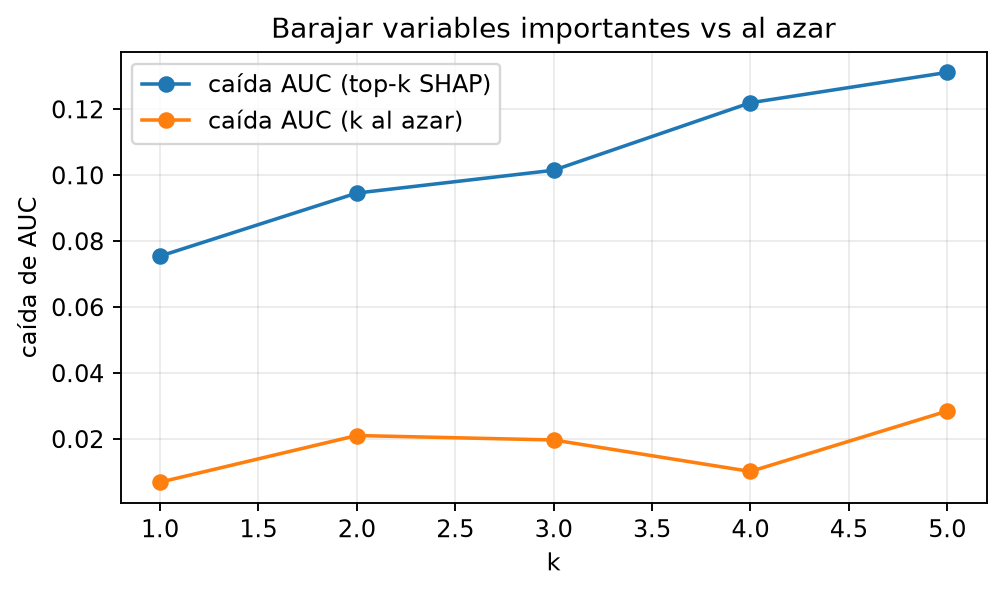
\includegraphics[width=0.45\linewidth]{figures/06_barajar_topk.png}
  \caption{Caída de AUC al barajar las $k$ variables más importantes según SHAP frente a $k$ variables al azar (sin reentrenar, la curva del azar es la media de 15 sorteos).}
  \label{fig:topk}
\end{figure}

%------------------------------------------------------------------
\section{Acciones e insights}
\subsection{Mejora del modelo guiada por las explicaciones}
Las explicaciones me dan dos ideas. Primero, las facturas \var{BILL_AMT2} a \var{BILL_AMT6} están muy correlacionadas con \var{BILL_AMT1} (0,89 de media) y cada una aporta poco ($<0{,}05$ de mean$|$SHAP$|$), así que son candidatas a quitar (\var{BILL_AMT1} sí importa y se queda). Segundo, el modelo vive del historial de pagos pero no tiene variables resumen, así que creo cuatro: utilización del límite, ratio pagado sobre factura, número de meses con retraso y retraso máximo. Las dos son hipótesis y la tabla~\ref{tab:mejora} las contrasta con el mismo protocolo y un bootstrap pareado.

\begin{table}[htbp]
\centering\small
\caption{Variantes del modelo (test). IC95\,\% del $\Delta$AUC con bootstrap pareado.}\label{tab:mejora}
\begin{tabular}{lrrrrrl}
\toprule
Variante & $n$ feat. & AUC val & AUC test & PR-AUC & Brier & $\Delta$AUC [IC95\,\%] \\
\midrule
Base & 22 & 0,7866 & 0,7731 & 0,5548 & 0,1356 & -- \\
A: sin \var{BILL_AMT2..6} & 17 & 0,7867 & 0,7735 & 0,5553 & 0,1357 & $+0{,}0004$ [$-0{,}0016$; $+0{,}0024$] \\
B: A + features nuevas & 21 & 0,7902 & 0,7770 & 0,5565 & 0,1354 & $+0{,}0039$ [$+0{,}0006$; $+0{,}0072$] \\
\bottomrule
\end{tabular}
\end{table}

Quitar las facturas no cambia nada, o sea el modelo se simplifica (cinco variables menos) sin perder rendimiento. Las features nuevas dan una mejora real pero pequeña (el IC no contiene el 0 aunque por muy poco) y casi nada en PR-AUC y Brier, lo cual tiene sentido porque los árboles ya podían combinar los \var{PAY_*}. Ojo con esto último porque el bootstrap pareado solo recoge la variabilidad del test y no la del entrenamiento. En el SHAP de la variante B (figura~\ref{fig:antes}) \var{MAX_RETRASO} y \var{N_MESES_RETRASO} entran en segunda y tercera posición y \var{UTIL_1} en quinta, mientras \var{PAY_0} baja de 0,48 a 0,39 y \var{PAY_2} sale del top-8. No es que importen menos sino que las variables derivadas se reparten el mérito con las originales. La utilización absorbe parte del papel de \var{LIMIT_BAL} (de 0,16 a 0,11) pero no el de \var{BILL_AMT1}, así que mi sospecha de que esta última capta la utilización solo se cumple a medias. Si priorizo simplicidad me quedo con A y si priorizo el AUC con B.

\begin{figure}[htbp]
  \centering
  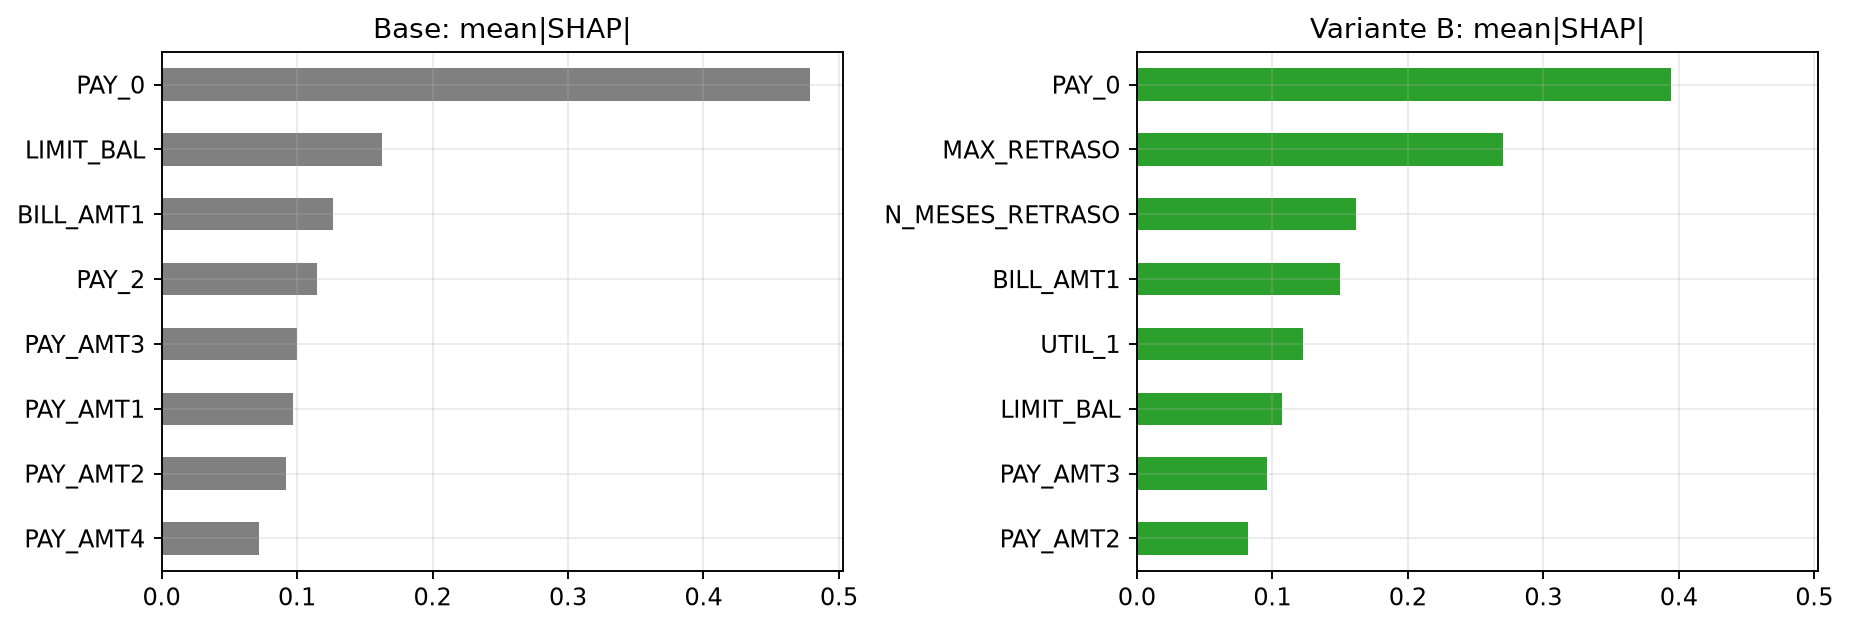
\includegraphics[width=0.85\linewidth]{figures/07_shap_antes_despues.png}
  \caption{Importancia SHAP antes (modelo base) y después (variante B).}
  \label{fig:antes}
\end{figure}

\subsection{Conclusiones de negocio}
El riesgo sale bien ordenado y calibrado por deciles (figura~\ref{fig:deciles}): el impago observado va del 4,5\,\% en el decil más bajo al 69,8\,\% en el más alto y el 10\,\% más arriesgado impaga 3,2 veces más que la media. Sirve para clasificar en bandas de riesgo y no solo para decir sí o no.

\begin{figure}[htbp]
  \centering
  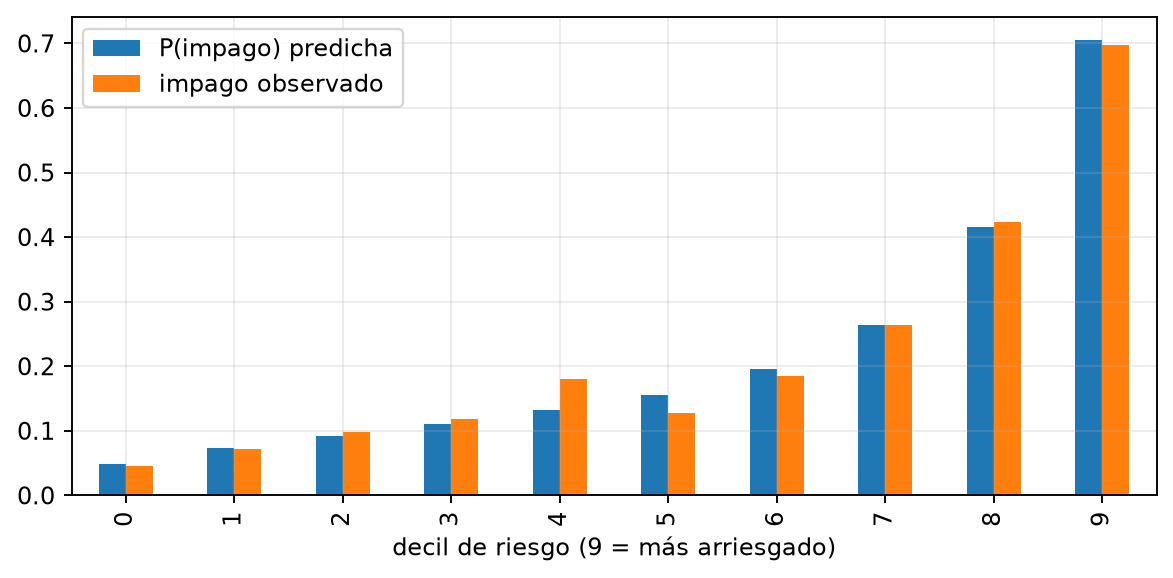
\includegraphics[width=0.45\linewidth]{figures/08_deciles.png}
  \caption{Probabilidad predicha frente a impago observado por deciles de riesgo (test).}
  \label{fig:deciles}
\end{figure}

El umbral es una decisión de negocio y cambia según lo que cueste un impago no detectado frente a una falsa alarma. Los costes de la tabla~\ref{tab:coste} son un supuesto mío y no datos del banco. Con 2:1 el modelo reduce el coste por cliente un 29\,\% respecto a aprobar a todos y con 5:1 un 29\,\% respecto a rechazar a todos. Con 10:1 el umbral cae a 0,09, se marca al 76\,\% de los clientes y el modelo apenas mejora a rechazar a todos (8\,\%), o sea que si equivocarse con un impago cuesta tanto el modelo aporta poco.

\begin{table}[htbp]
\centering\small
\caption{Política por coste (test). Coste por cliente con una falsa alarma igual a 1.}\label{tab:coste}
\begin{tabular}{lrrrrr}
\toprule
Coste FN:FP & Umbral (val) & Con modelo & Aprobar a todos & Rechazar a todos & \% marcado \\
\midrule
2:1 & 0,27 & 0,313 & 0,443 & 0,779 & 24,1 \\
5:1 & 0,18 & 0,555 & 1,106 & 0,779 & 37,9 \\
10:1 & 0,09 & 0,718 & 2,213 & 0,779 & 76,1 \\
\bottomrule
\end{tabular}
\end{table}

Por segmentos, el 23\,\% de los clientes ya va con retraso y de ellos impaga el 50\,\%, frente al 14\,\% de los que van al día. En los morosos el modelo casi solo lee el historial (\var{PAY_0} con 0,72 y \var{PAY_2} con 0,26 de mean$|$SHAP$|$) y en los que van al día pesan más \var{LIMIT_BAL}, \var{BILL_AMT1} y los pagos, con \var{PAY_2} en 0,07. Esto importa porque el 48,5\,\% de los impagos (en validación) sale de clientes que van al día, justo los que tienen señales más flojas. Sugiere políticas distintas: cobro y renegociación para los morosos y vigilar la utilización del límite y los pagos en el resto.

\subsection{Equidad y sesgos}\label{sec:equidad}
Aunque el sexo no entra como variable audito el modelo en test con el umbral global (tabla~\ref{tab:equidad}). A los hombres se les marca más (26,4\,\% frente a 22,6\,\%) pero también impagan más (24,4\,\% frente a 20,7\,\%), sufren más falsas alarmas (FPR de 0,174 frente a 0,137) y el modelo discrimina peor en ellos (AUC de 0,754 frente a 0,786) mientras que el recall es parecido. Por edad las brechas son mayores: el recall va de 0,517 en 30 a 39 años a 0,648 en 50 o más (grupo pequeño, 560 clientes). El SHAP por sexo es casi idéntico (\var{PAY_0} con 0,49 en hombres y 0,47 en mujeres), así que el modelo usa la misma evidencia para los dos y las diferencias vienen de las distribuciones. Predecir el sexo con el resto de variables da un AUC de 0,64, un proxy flojo-moderado, o sea que quitar la variable no elimina toda la información sobre ella.

Como mitigación pruebo un umbral por sexo (0,281 hombres y 0,252 mujeres) ajustado en validación para igualar el recall, en la línea de \citet{hardt2016}. La brecha de FPR baja de 0,037 a 0,007 y la de porcentaje de marcados de 0,038 a 0,009 sin cambiar el F1, pero la brecha de recall, que era lo que quería igualar, sube de 0,023 a 0,053. Creo que es ruido de muestreo (con unos 570 positivos en hombres y 760 en mujeres el error típico de esa diferencia ronda 0,03, cuenta aproximada mía) y lo cuento tal cual. Además usar el sexo para decidir es discriminación directa, así que lo planteo como experimento y no como recomendación. Por último, quitar edad, estado civil y educación solo baja el AUC de test de 0,7731 a 0,7707, aunque no he medido si eso reduce las brechas.

\begin{table}[htbp]
\centering\small
\caption{Auditoría por sexo en test, antes y después del umbral por sexo.}\label{tab:equidad}
\begin{tabular}{llrrrrrr}
\toprule
 & Grupo & \% marcados & TPR & FPR & Brecha TPR & Brecha FPR & F1 \\
\midrule
\multirow{2}{*}{Antes} & hombre & 0,264 & 0,545 & 0,174 & \multirow{2}{*}{0,023} & \multirow{2}{*}{0,037} & \multirow{2}{*}{0,534} \\
 & mujer & 0,226 & 0,568 & 0,137 & & & \\
\midrule
\multirow{2}{*}{Después} & hombre & 0,252 & 0,536 & 0,161 & \multirow{2}{*}{0,053} & \multirow{2}{*}{0,007} & \multirow{2}{*}{0,535} \\
 & mujer & 0,243 & 0,589 & 0,153 & & & \\
\bottomrule
\end{tabular}
\end{table}

%------------------------------------------------------------------
\section{Discusión}
\paragraph{Qué explicaciones aguantan.} SHAP pasa los chequeos y es estable en las primeras posiciones del ranking (historial de pagos, límite y \var{BILL_AMT1}) aunque en la cola es menos fiable. LIME es el punto débil y yo lo usaría como apoyo y no como confirmación.

\paragraph{Dónde pueden engañar.} Con variables correlacionadas la permutación puede infravalorar y SHAP repartir el mérito entre variables parecidas \citep{kumar2020}, como se ve con \var{PAY_2} y en la variante B. El PDP de \var{LIMIT_BAL} promedia clientes muy distintos. Y el verdadero y el falso positivo tienen casi la misma explicación y distinto resultado, así que una explicación no basta para saber si el modelo acierta.

\paragraph{Interpretaciones erróneas.} SHAP no es causalidad (\var{LIMIT_BAL} lo fija el banco) y un contrafactual que pide cambiar el pasado no le sirve de mucho al cliente: con riesgo alto ninguna de las acciones que probé lo saca de la lista.

\paragraph{Límites.} Los datos son de Taiwán de 2005 y no representan a un banco europeo de hoy. Hay un solo corte con partición aleatoria (en producción haría falta validación temporal), los costes FN:FP son un supuesto y la mejora de la variante B es pequeña y su intervalo no recoge la variabilidad del entrenamiento.


\FloatBarrier
\bibliographystyle{unsrtnat}
\bibliography{references}

\end{document}
